\subsection{Microbiota dataset}

As we look into the microbiota data, we notice a major phylogenetic architecture to describe various levels of precision in the microbiota composition.
Indeed, such phylogenetic structure can be represented as a tree as on the following figure:
\begin{figure}[H]
    \center
    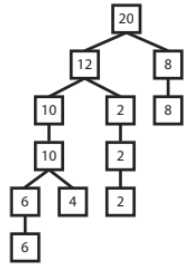
\includegraphics[scale=1]{images/abundance_tree_phylogenetic}
    \caption{Phylogenetic tree example with abundance data (in the nodes) at each layer of the tree.
    Each node represents a bacterium specie at a given precision layer in the tree. From \cite{microbiome_deeplearning_research}.}
    \label{fig:phylogenetic_tree}
\end{figure}

Such structure can not be used directly in a machine learning system since it's not a vectorizable representation.
Hence, we first suggest to transform the tree in a matrix to image structure as in the following example:
\begin{figure}[H]
    \center
    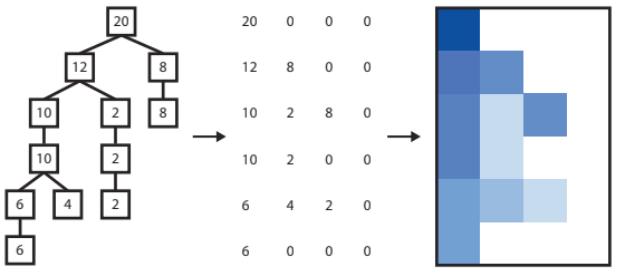
\includegraphics[scale=1]{images/tree_to_image}
    \caption{Phylogenetic tree to image representation:
    opacity of the pixel relates to the abundance of the species at the given level of precision (normalized between 0 and 1).
    From \cite{microbiome_deeplearning_research}.}
    \label{fig:phylogenetic_tree_to_img}
\end{figure}

Sadly this image representation does not convey the link between the species abundance given by the edges of the tree.
As a result, we suggest to find a hidden variable $Z$ that uses the adjacent matrix of the tree $T$, to find a way to go through the image
as for the PixelCNN approach.
Such approach, in addition to use the adjacency of the tree graph, would then learn an interesting trajectory to compute the correlation between the abundance data.
The next section offers the mathematical framework of the proposed idea.